\documentclass{article}
\usepackage[margin=1in]{geometry}
\usepackage{graphicx}
\usepackage{caption}
\usepackage{color}
\usepackage{subcaption}
\usepackage{hyperref}
\graphicspath{ {/asay/Desktop/images/} }
\usepackage{xepersian}




\title{پاسخ تمرین شماره ۲
	\lr{\textcolor{red}{gem5}}
	\\
	 درس معماری کامپیوتر }


\author{امیر حسین عاصم یوسفی \\ ۹۶۱۱۰۳۲۳}
\settextfont{B Nazanin}
\begin{document}
	\maketitle
	برای انجام این آزمایش از برنامه
	\lr{Hanoi Tower}
	با مقدار ورودی ۱۵ استفاده شده است که اجرای آن تقریبا ۵ دقیقه و ۲۶ ثانیه طول می کشد  و کد آن به پیوست ارسال شده است  . \\
برای این که برنامه بر روی 
\lr{Config File }
ای که طراحی کرده ایم اجرا شود باید از دستور زیر استفاده کرد  : 
\begin{center}
	\lr{./build/X86/gem5.opt configs/example/MyConfig.py -c mytest/a.out}
\end{center}
که نتایج اجرا برای هرکدام از 
\lr{Config}
های مختلف به صورت زیر است  . 
\begin{center}

	
	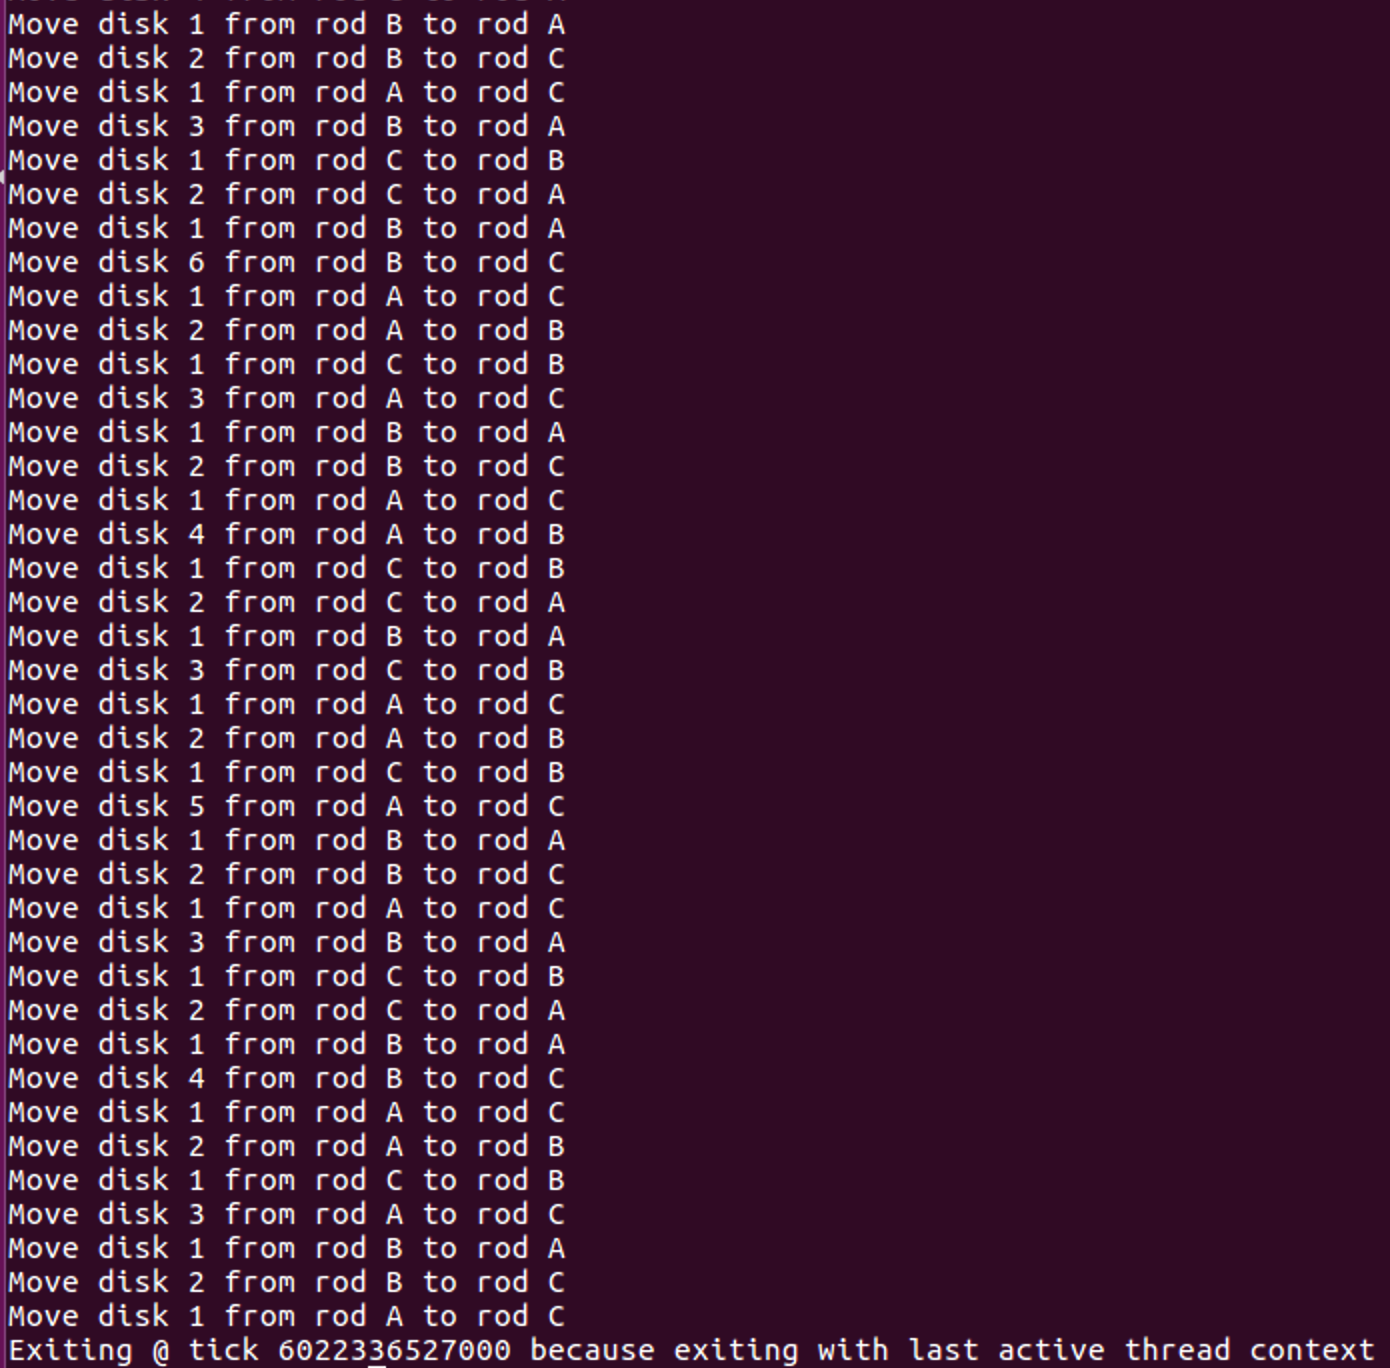
\includegraphics[width=.4\linewidth]{firstConfigSim} 
		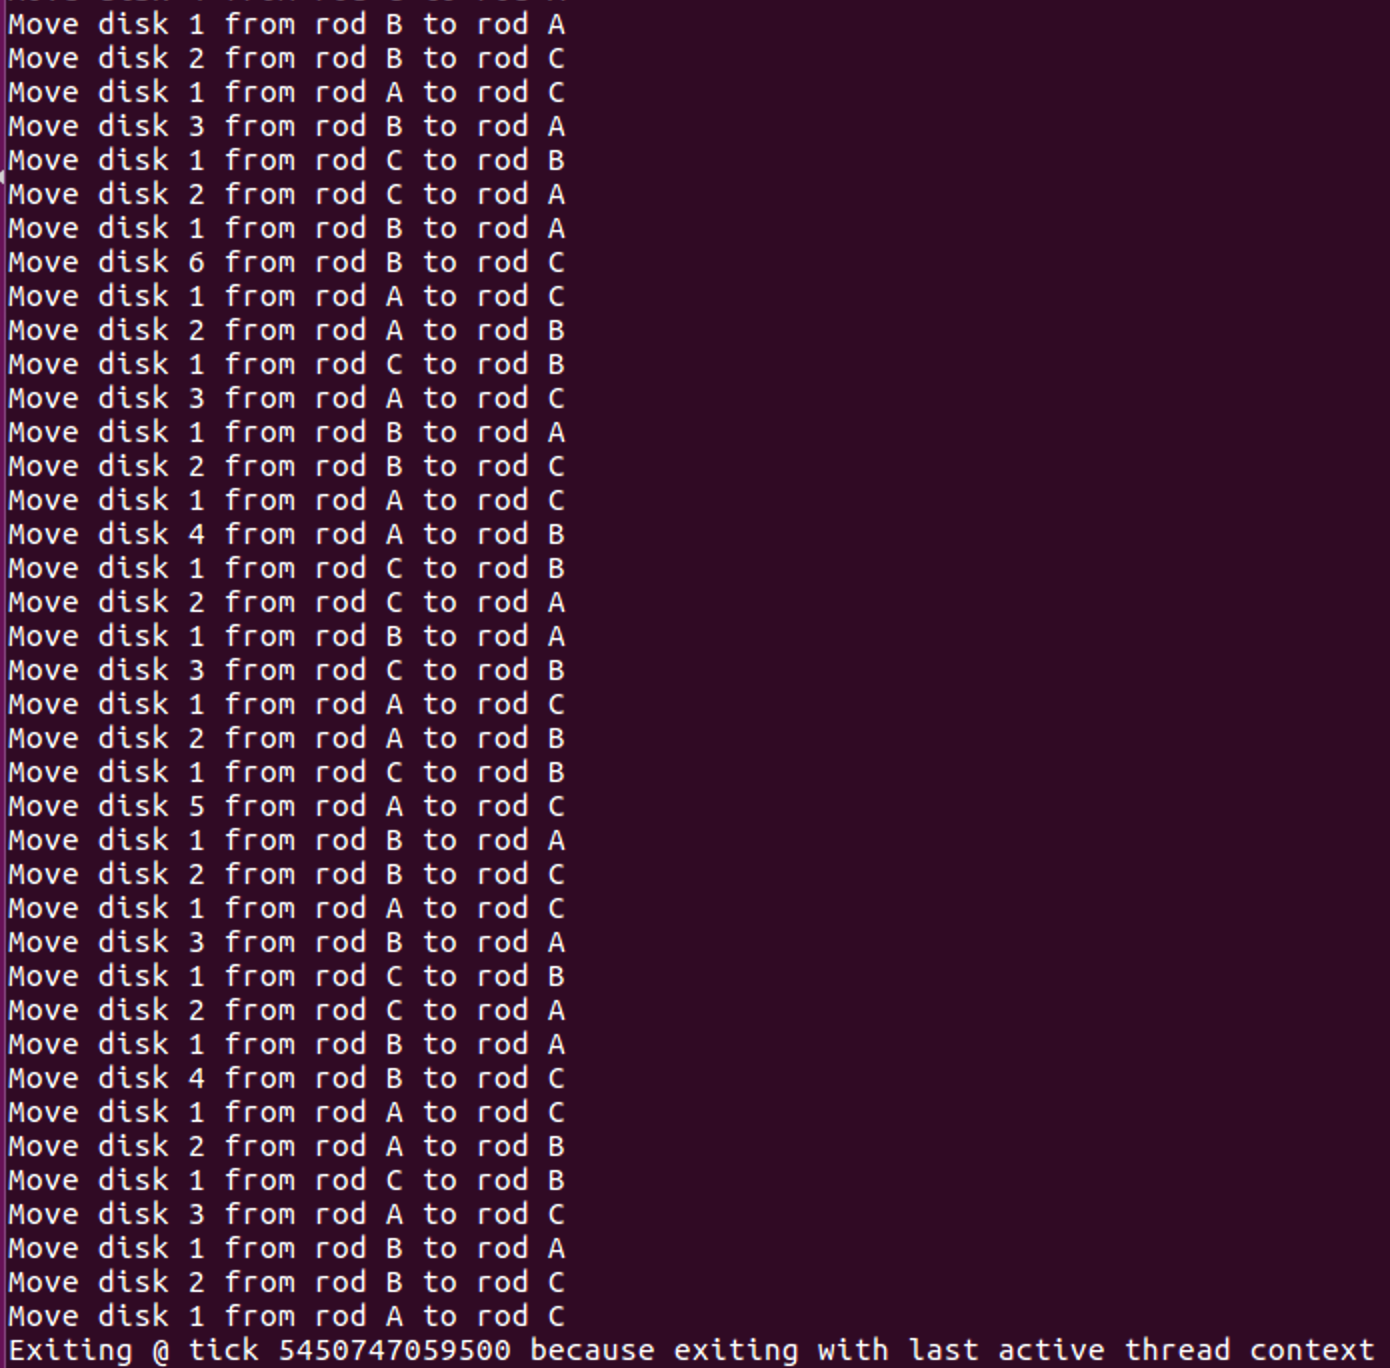
\includegraphics[width=.4\linewidth]{secondConfigSim} 
			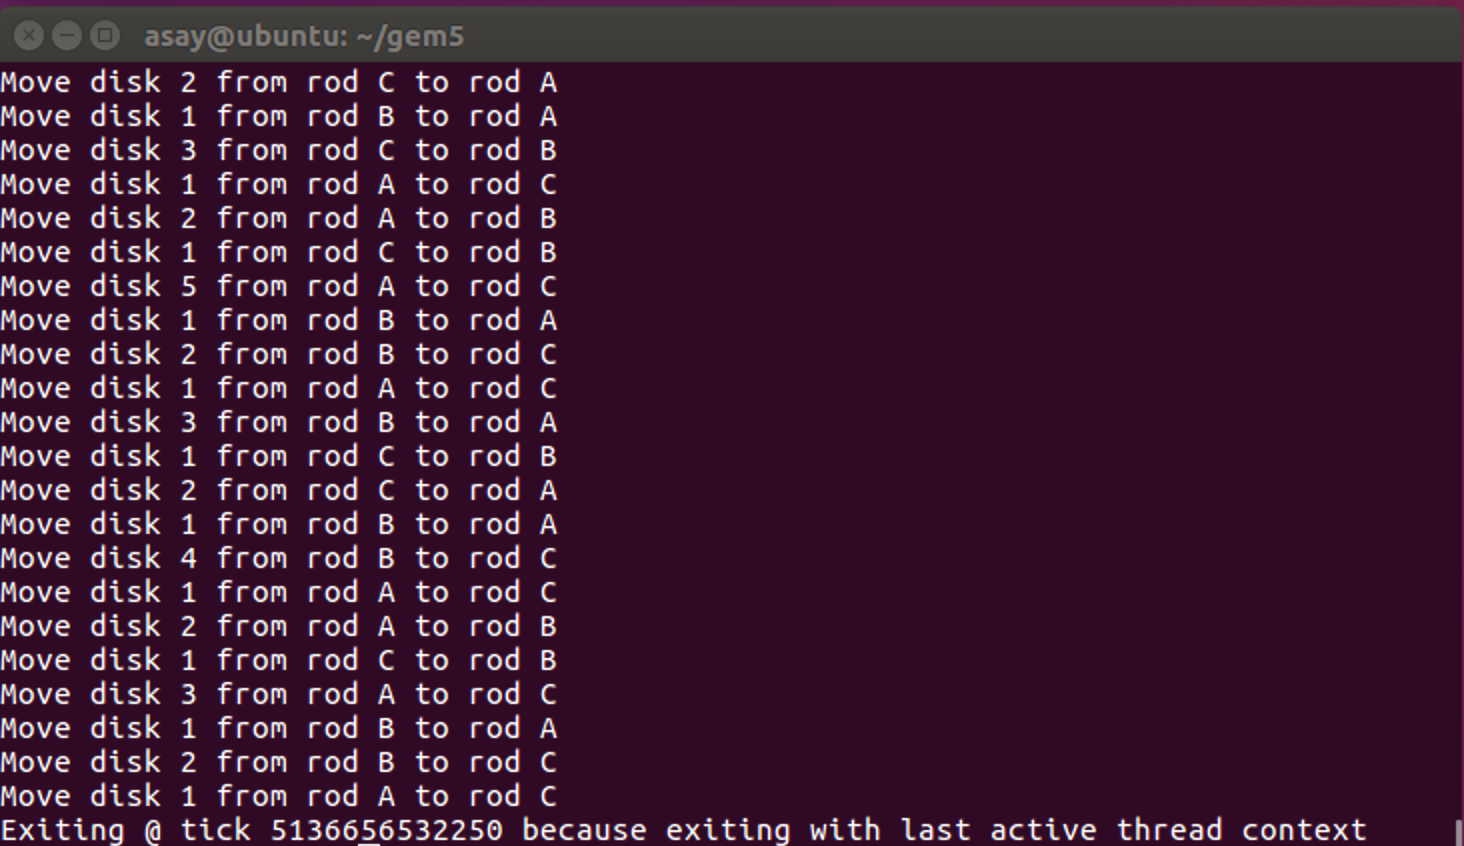
\includegraphics[width=.4\linewidth]{thirdConfigSim} 
			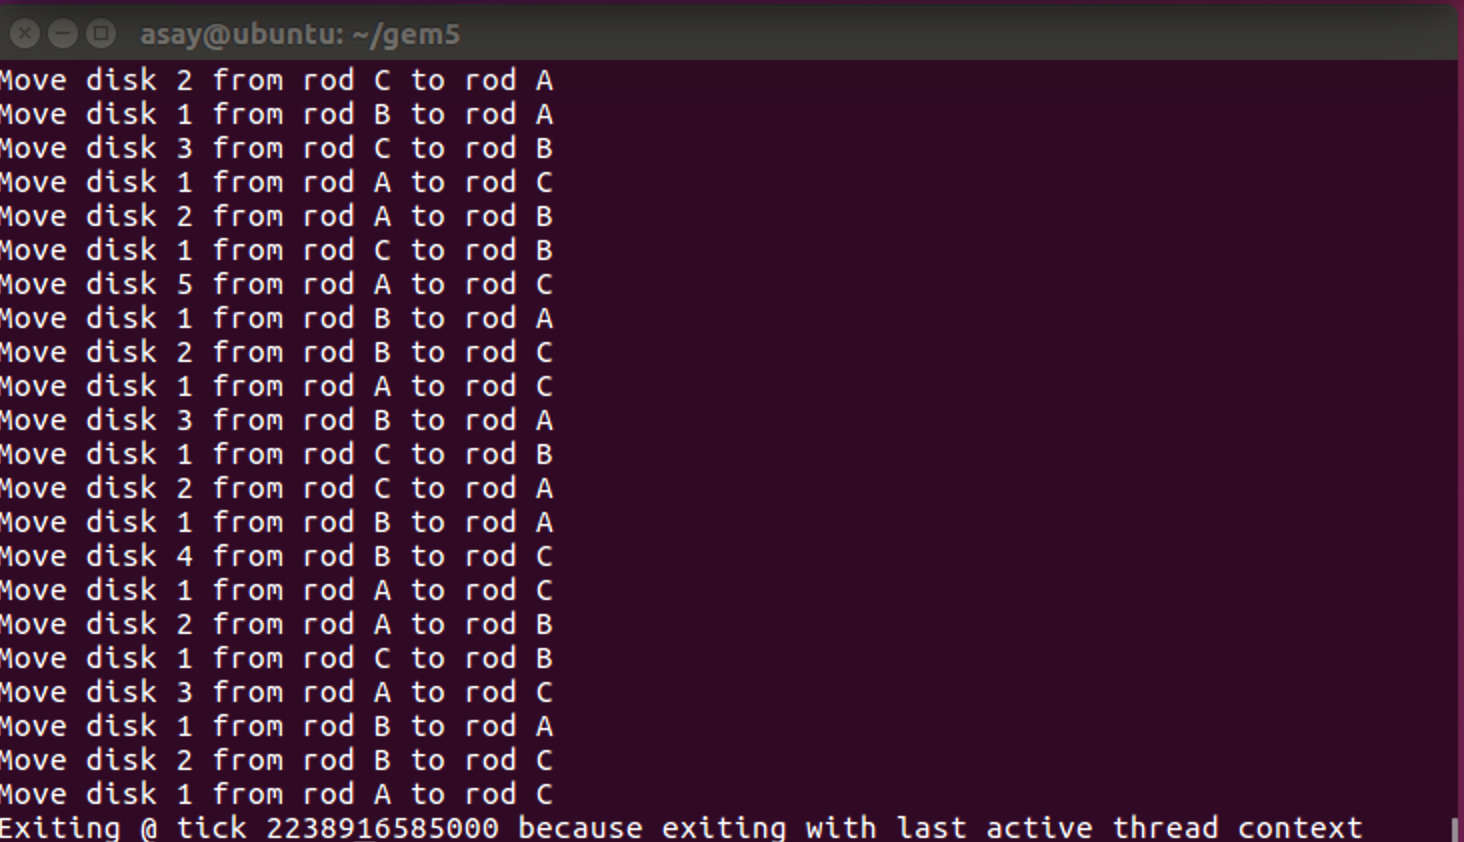
\includegraphics[width=.4\linewidth]{forthConfigSim} 
			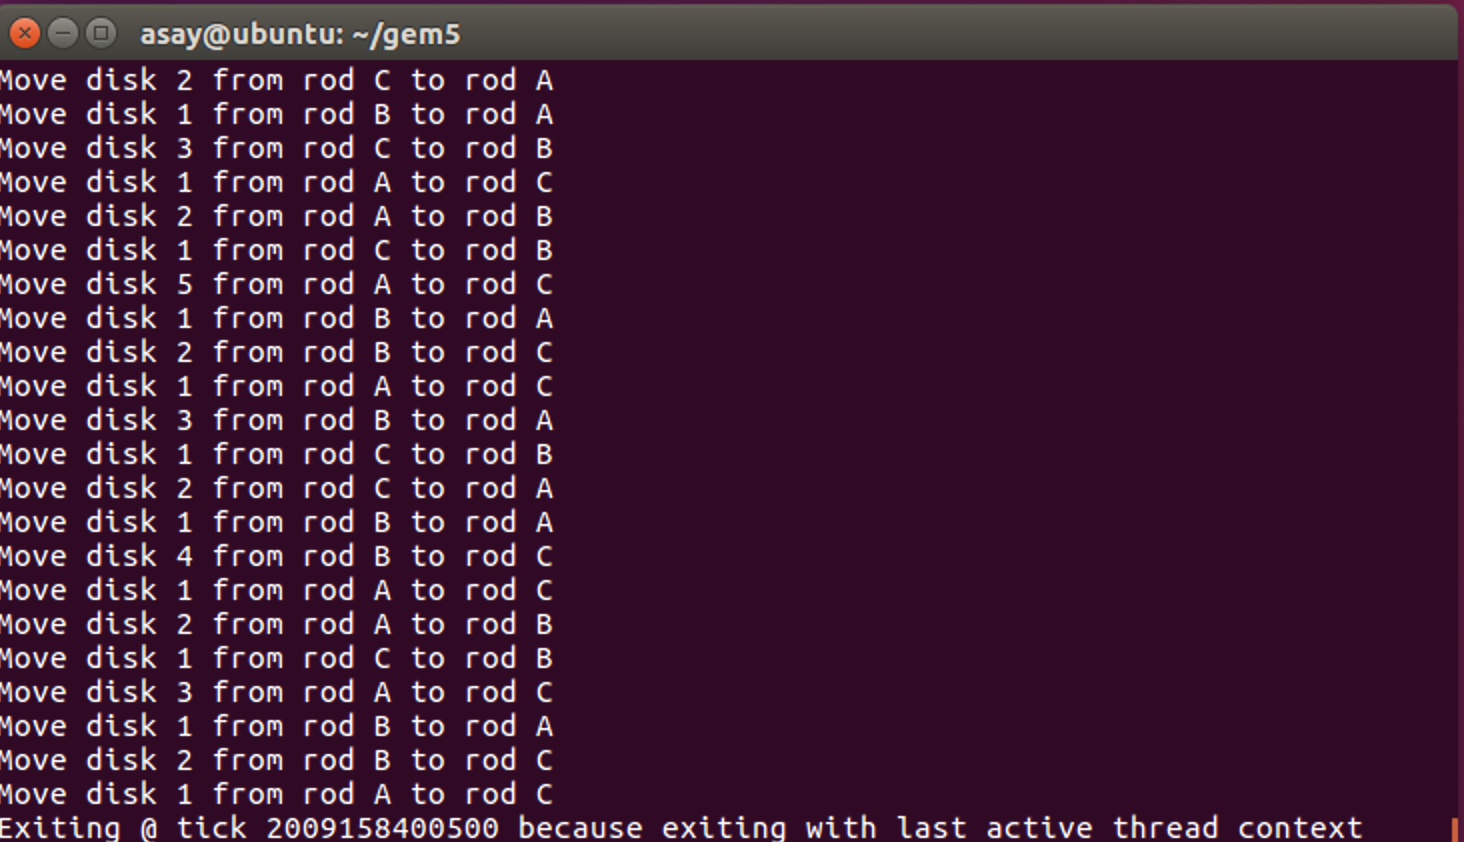
\includegraphics[width=.4\linewidth]{fifthConfigSim} 
			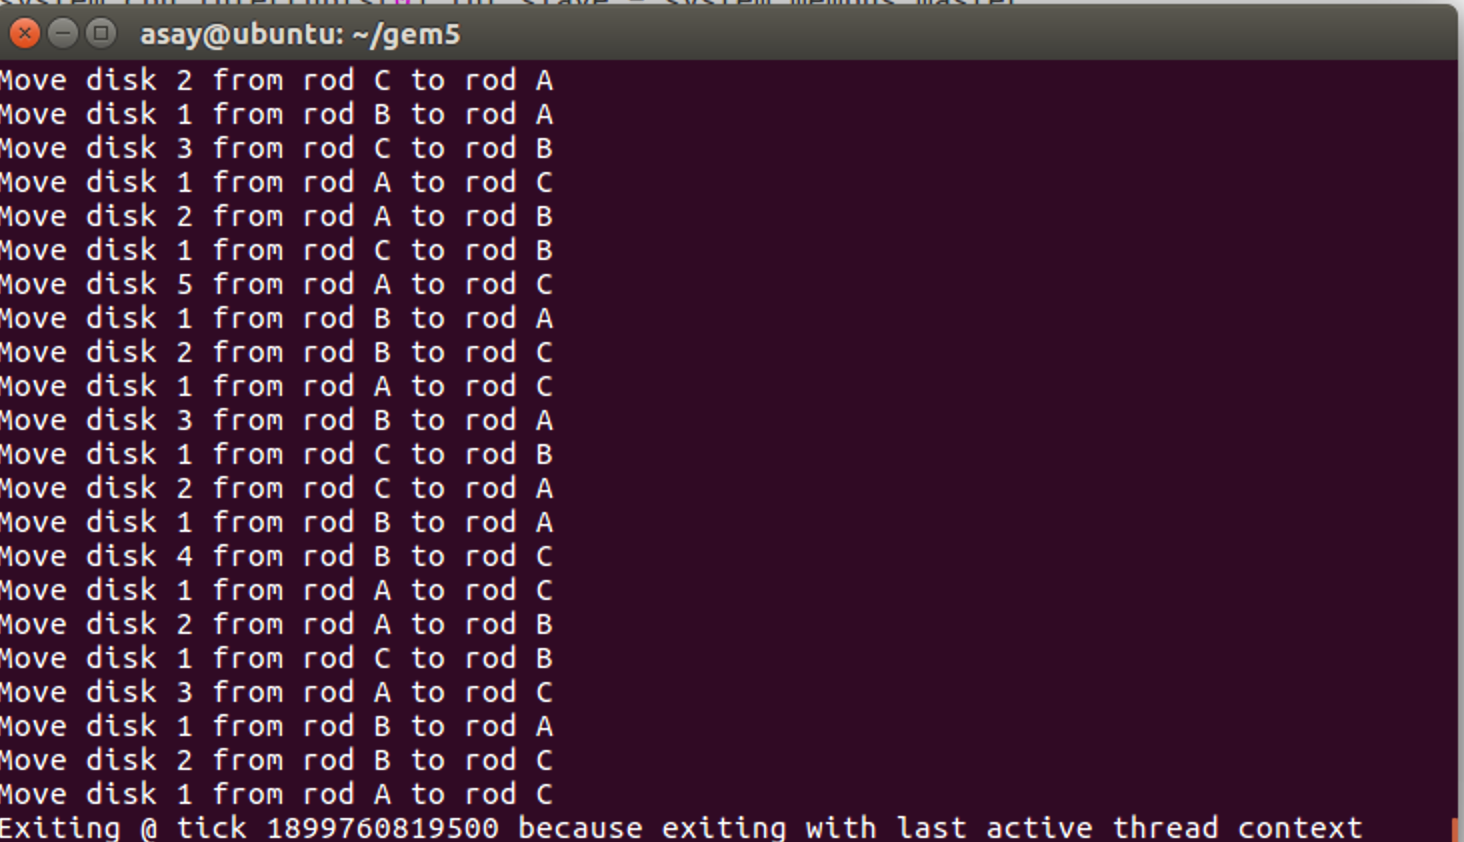
\includegraphics[width=.4\linewidth]{sixthConfigSim} 
			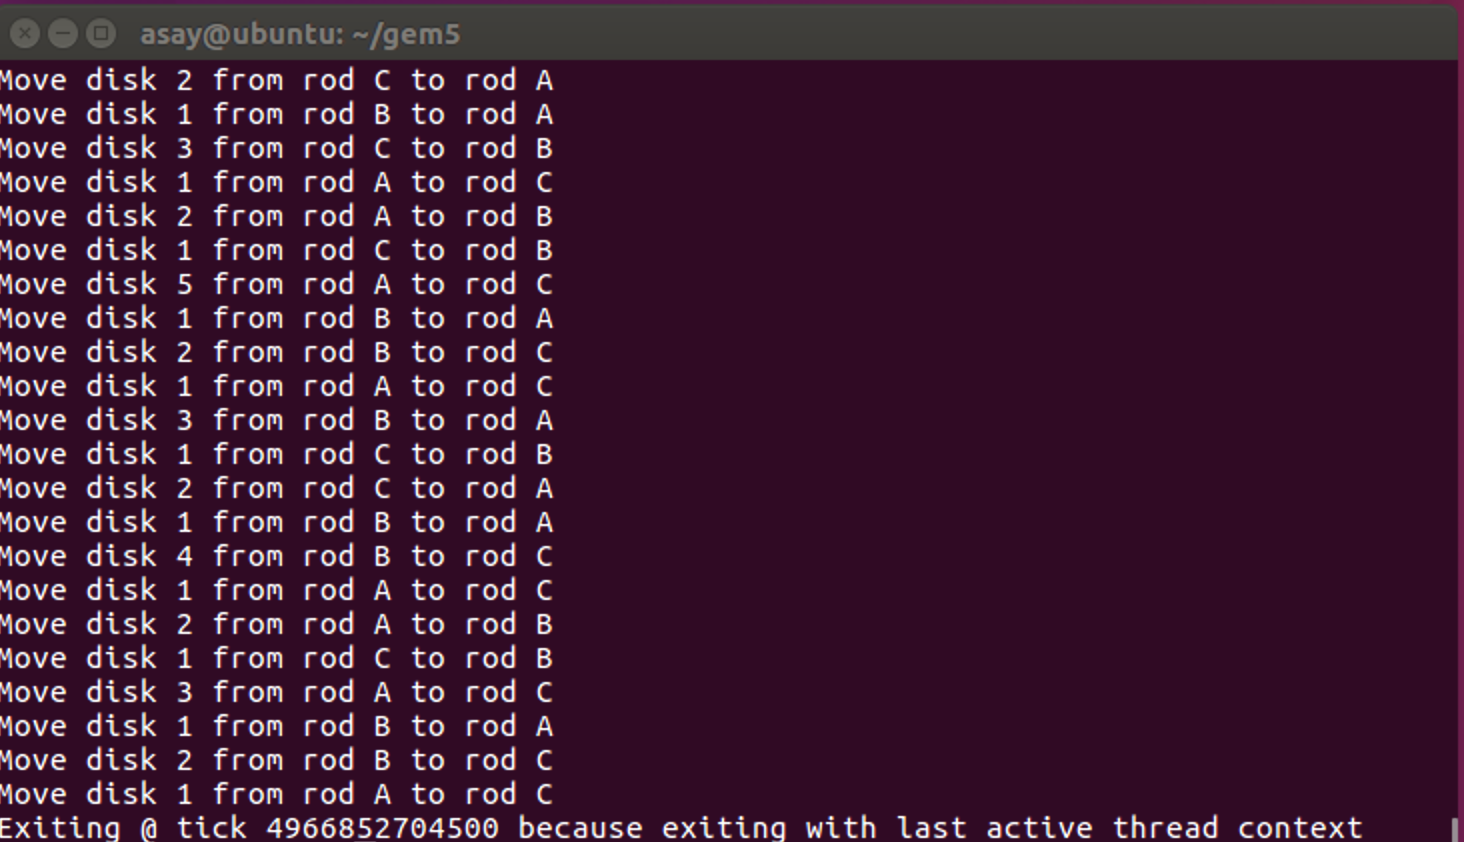
\includegraphics[width=.4\linewidth]{seventhConfigSim} 
			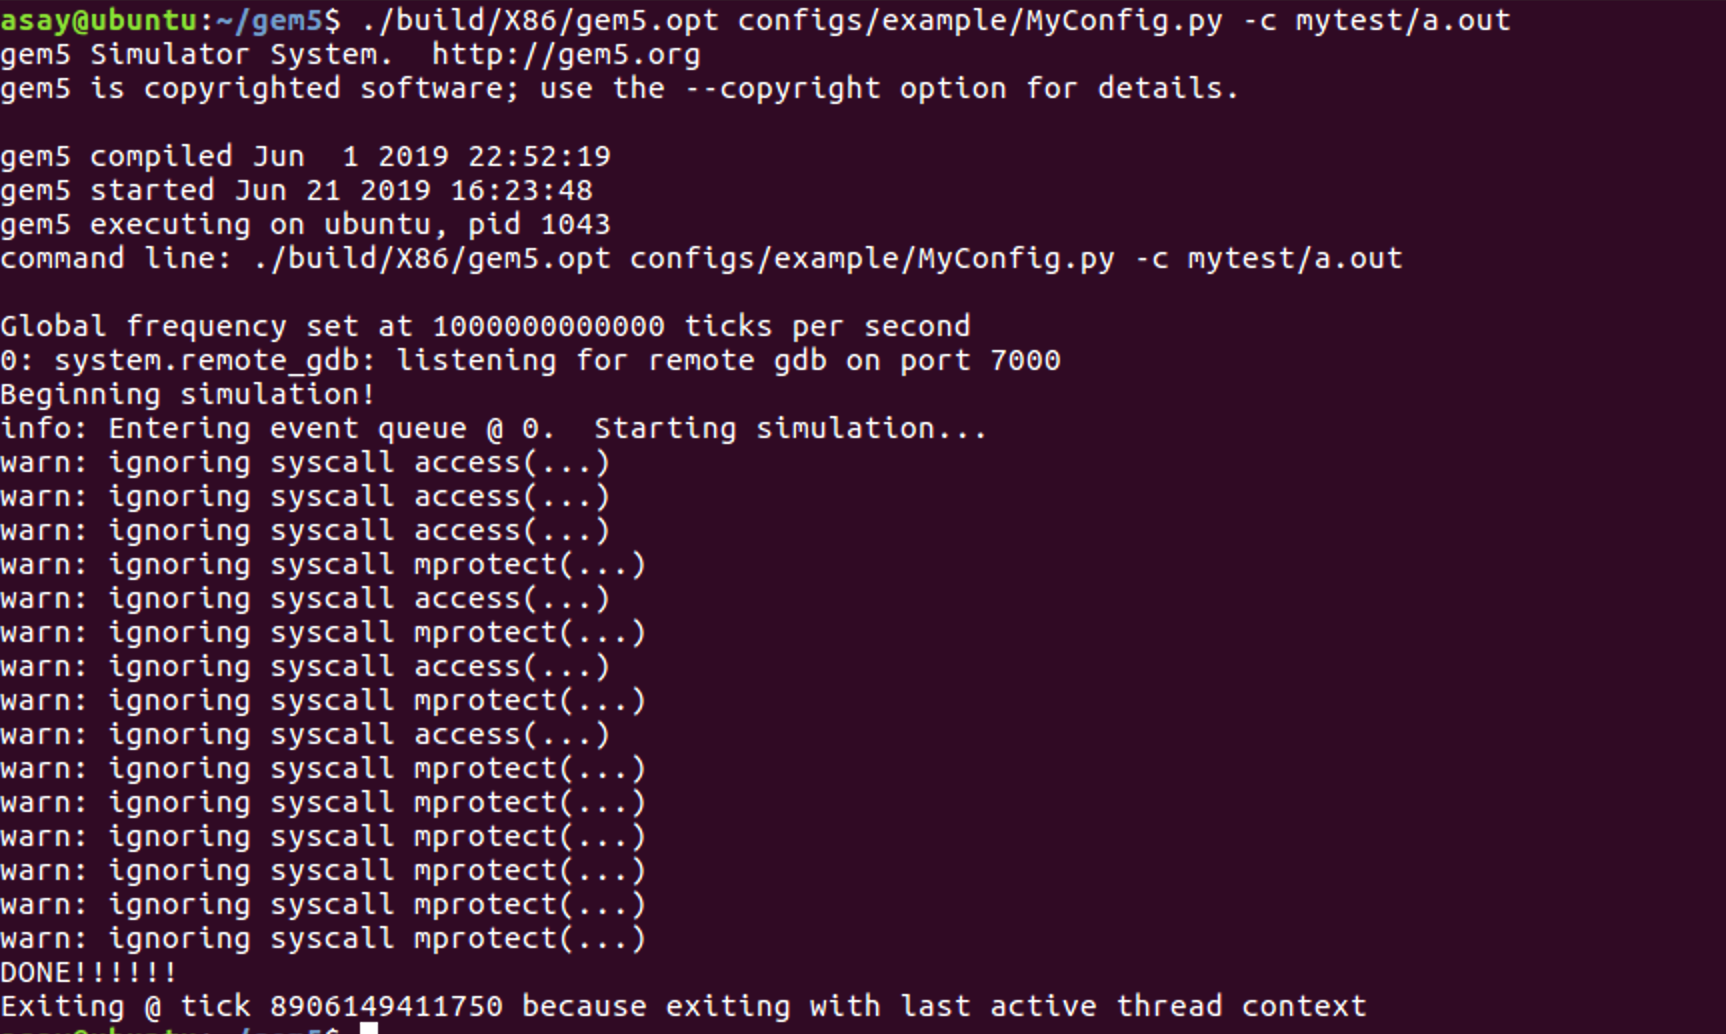
\includegraphics[width=.4\linewidth]{8thConfigSim} 
			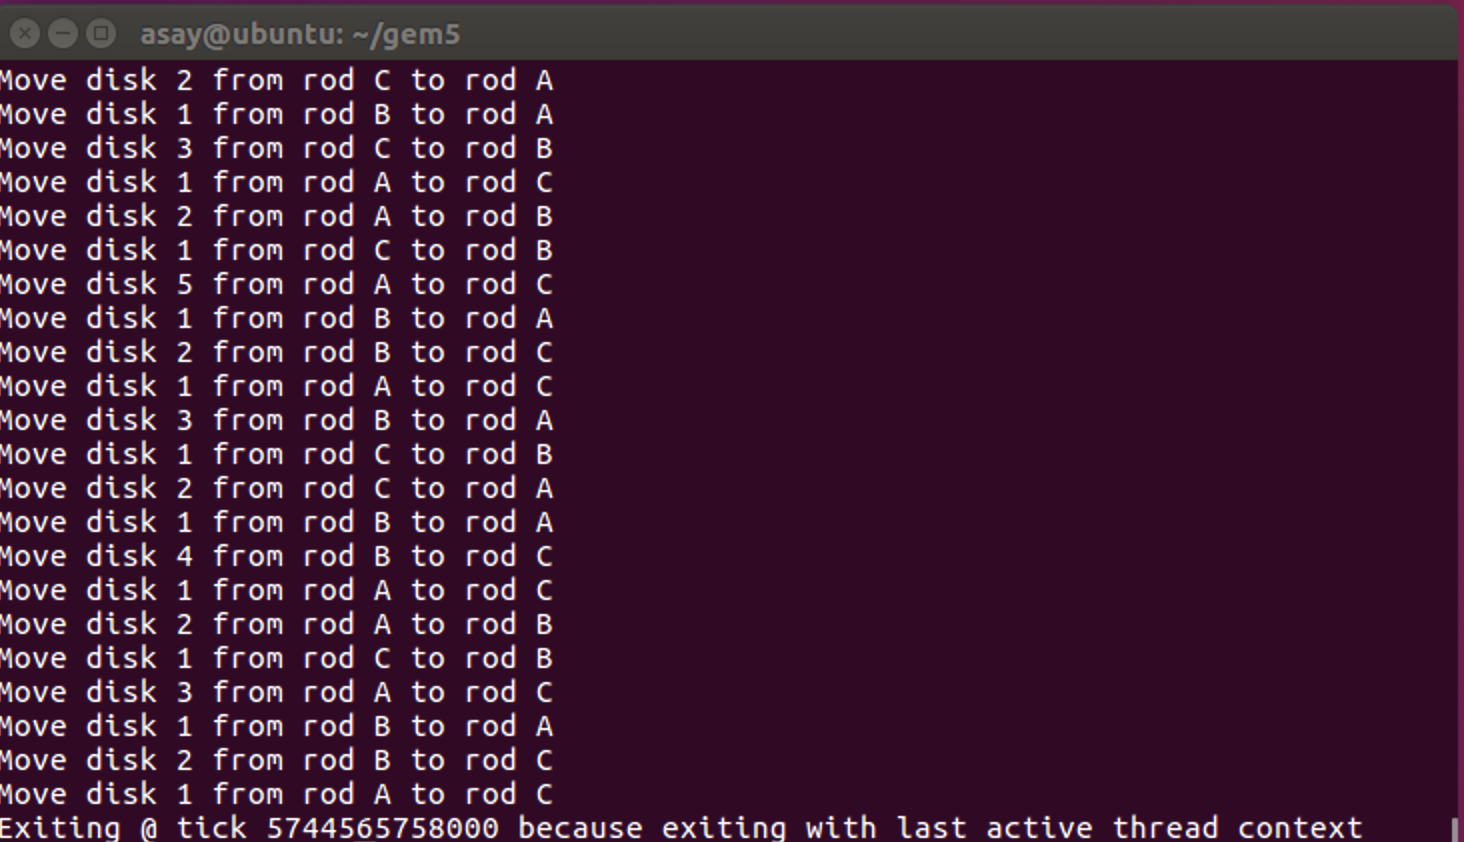
\includegraphics[width=.4\linewidth]{9thConfigSim} 
			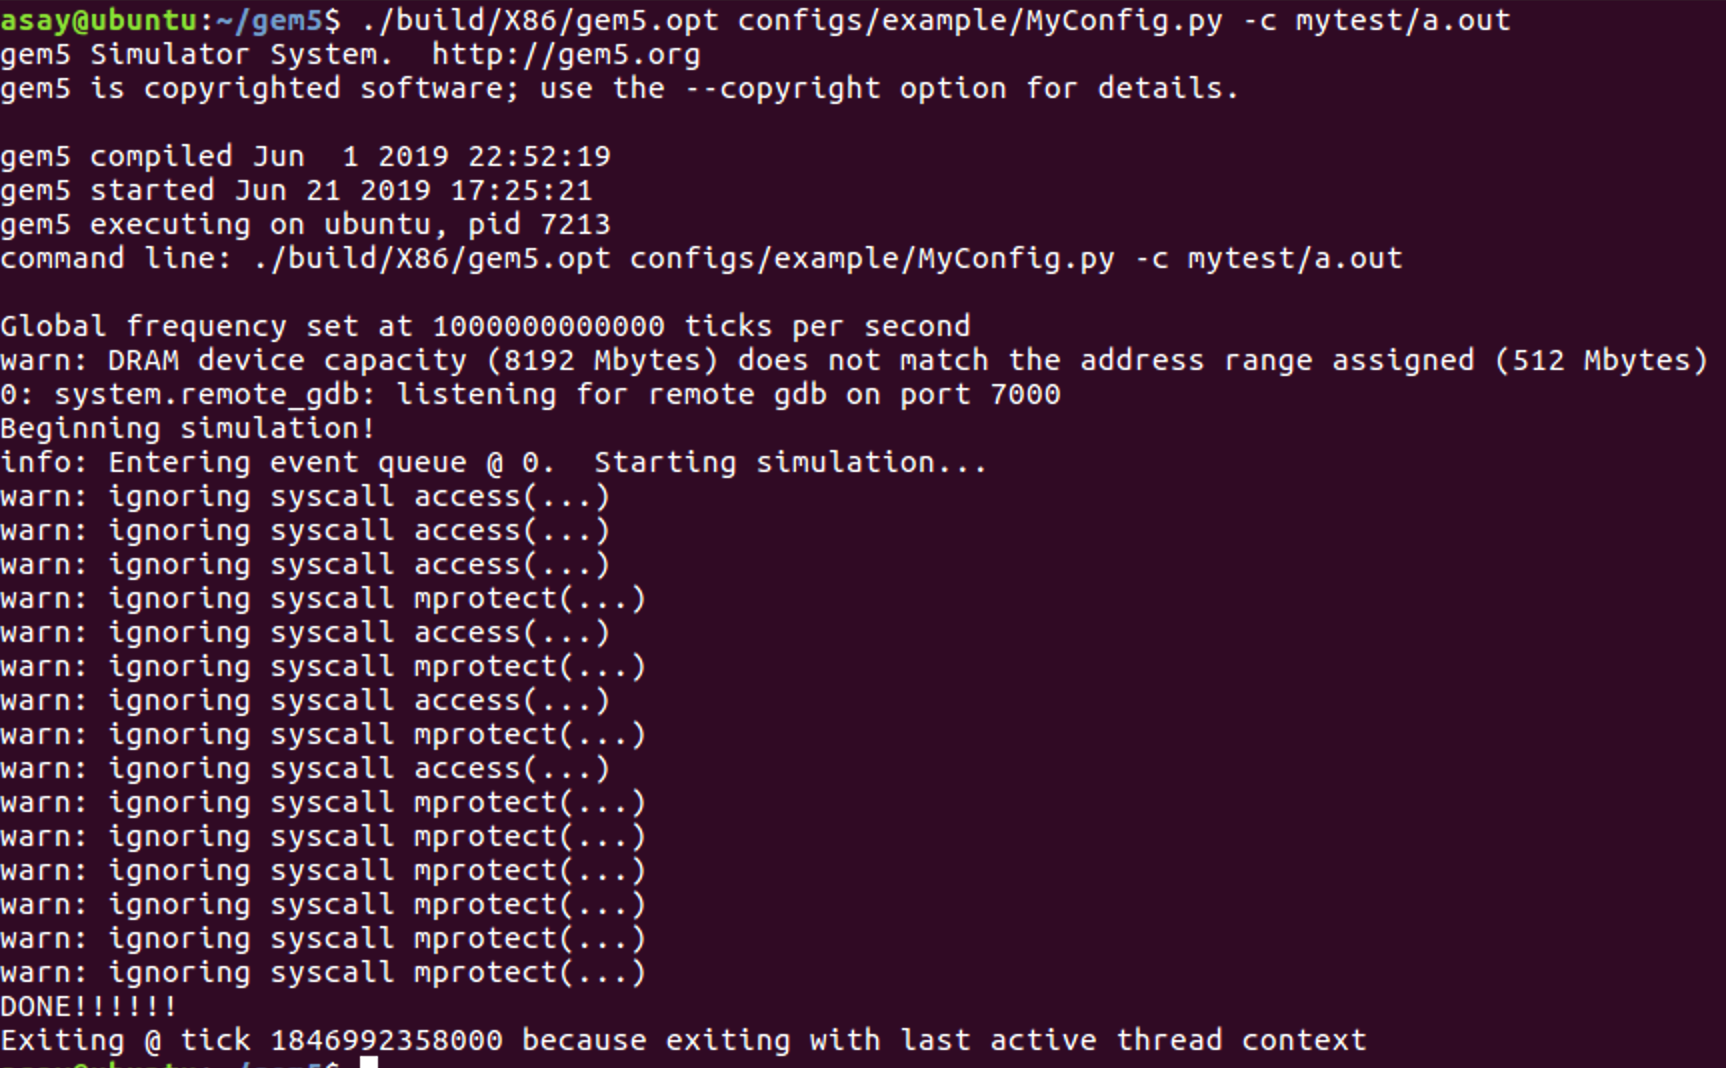
\includegraphics[width=.4\linewidth]{10thConfigSim} 
			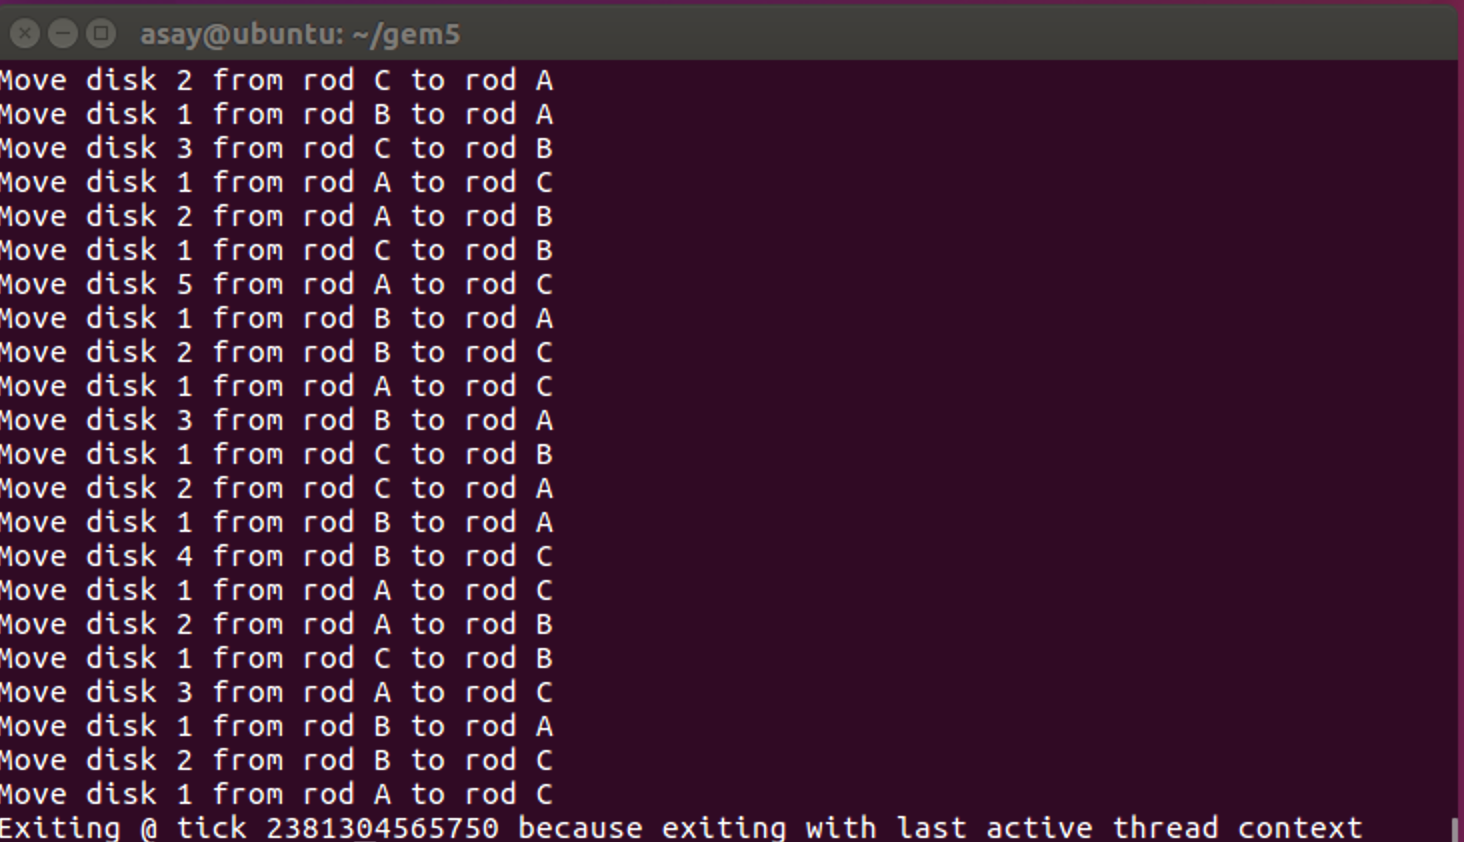
\includegraphics[width=.4\linewidth]{11thConfigSim} 
			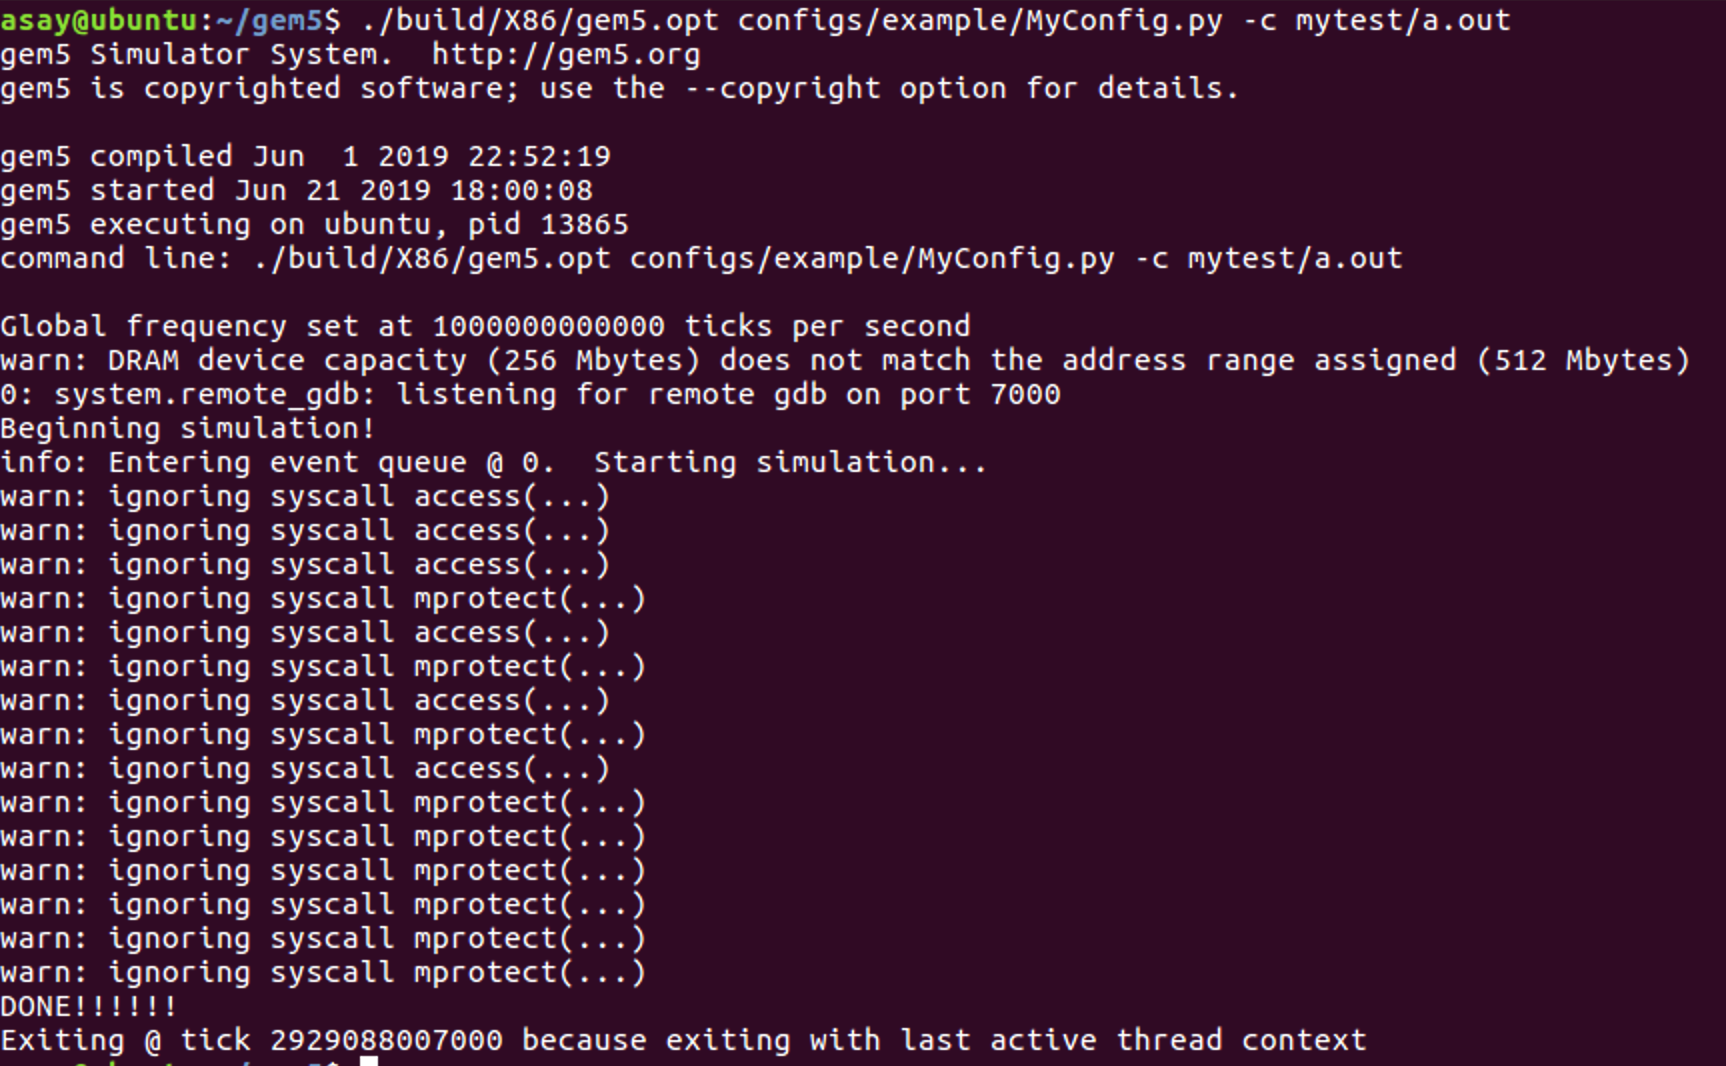
\includegraphics[width=.4\linewidth]{12thConfigSim} 


\end{center}
\section*{سوال ۱ }
برای ارزیابی کارکرد مدل های مختلف پردازنده می توان زمان اجرا 
\lr{ٍ(Execution Time)}
 را در نظر گرفت . 
علت آن هم این است که  زمان اجرا  به راحتی می تواند تفاوت در تغییر فرکانس و حافظه را به مانشان دهد \\
زیرا در صورتی که حافظه نتواند یک در خواست را در یک کلاک جواب دهد با توجه به حجم برنامه تاثیر به سزایی در زمان اجرا  دارد . \\
همچنین درمورد پردازنده اگر یک پرازنده نتواند عملیات ها خود را در مدت یک کلاک انجام دهد و نتیجه درست را بدهد می تواند با توجه به حجم برنامه تاثیر به سزایی در زمان اجرا  بگذارد . 
\section*{سوال۲ }
با توجه به معیار گفته شده در بالا می توان به جدول زیر رسید 
\begin{center}
				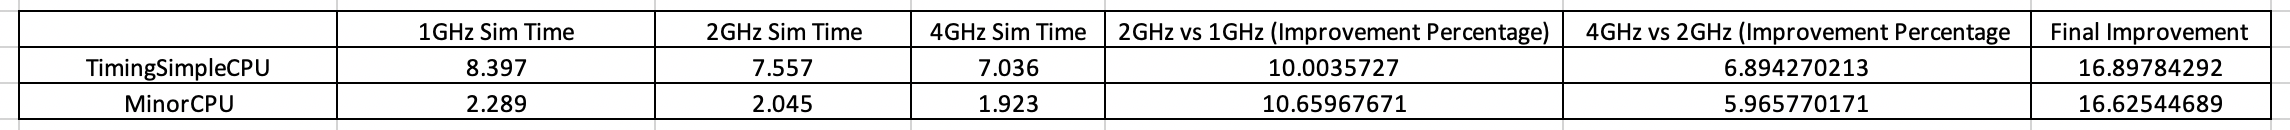
\includegraphics[width=1\linewidth]{q2p1} 
\end{center}
با توجه به جدول بالا می توان دید
\lr{\textcolor{red}{MinorCPU}}
بسیار حساس تر می باشد . \\
علتش تفاوت در ساختار این دو پردازنده می باشد زیرا در پردازنده حساس تر عملیات به صورت
\lr{pipeline}
 انجام میشه و بنابراین تغییر در فرکانس می تواند در طول هر 
\lr{step}
تاثیر بگذارد بنابراین درکل زمان اجرا را تغییر به سزایی می دهد  . 
\section*{سوال ۳}
با توجه به معیار گفته شده در سوال ۱ می توان به جدول زیر رسید 
\begin{center}
	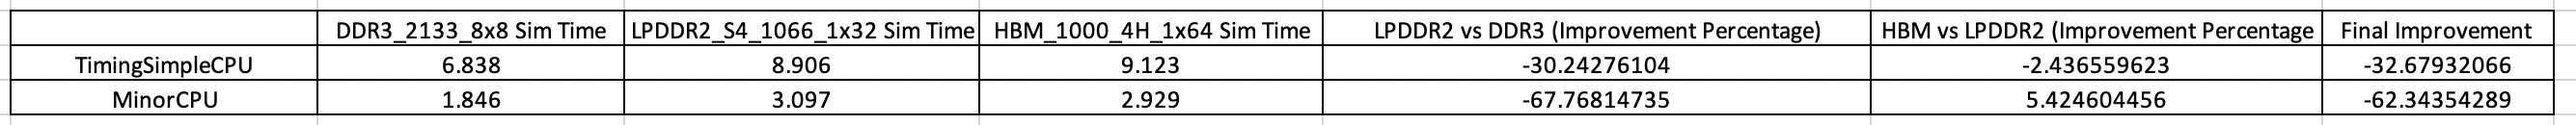
\includegraphics[width=1\linewidth]{q3p1} 
\end{center}

همان طور که می توان دید 
\lr{\textcolor{red}{TimingSimpleCPU}}
نسبت به تغییرات حافظه حساس تر است . \\
علت این که این مدل پردازنده حساس تر است به این دلیل که دسترسی های آن به حافظه بیشتر است بنابراین تغییرات در حافظه که منجر به تغییرات در زمان پاسخگویی حافظه به درخواست  های پردازنده می شود تاثیرات بیشترین بر روی این پردازنده دارد . 
\section*{سوال ۴}
نسبت به تغییرات 
\lr{CPU}
حساس تر است زیرا ساختار این دو پردازنده که یکی 
\lr{Pipeline}
و دیگری به صورت 
\lr{Multicycle}
می باشد بیشتری تاثیر را در زمان اجرا دارد . 
\section*{سوال ۵}
بله . زیرا هر برنامه تعداد منحصر به فرد دسترسی به حافظه و عملیات های پردازشی دارد بنابراین حتما نتایج آزمایش متفاوت خواهد بود . 


\end{document}